%\documentclass[10pt,a4paper,slovene,openany]{book}
\documentclass[oneside,a4paper,openany,12pt]{scrbook}
%\usepackage[a4,center,cam]{crop}
%\usepackage[slovene]{babel}
%\usepackage[T1]{fontenc}
%\usepackage[pdftex]{graphicx,thumbpdf}
%\usepackage{epstopdf}
%\usepackage[math]{kurier}

\newcommand {\e}[1]{\mathrm{~#1}}
\usepackage{paralist}
\usepackage{caption}

\setlength{\parskip}{1em}%
\setlength{\parindent}{0cm}

\usepackage{titling}
\usepackage{amsmath,amssymb,amsfonts,nicefrac}
\usepackage{graphicx}
\usepackage{color}
\usepackage{float}
\usepackage{mathtools}
\allowdisplaybreaks
\usepackage[pdftex,colorlinks=true,citecolor=blue,linkcolor=black,urlcolor=blue,bookmarks=true]{hyperref}
\usepackage{pifont}
\usepackage{dictsym}
\usepackage{braket}
\usepackage{slashed}
\DeclareMathOperator{\arcsinh}{arcsinh}
\include{definicije}
\usepackage{enumerate}

%\usepackage[utf8]{inputenc}
%\usepackage[titles]{tocloft}
%\usepackage{setspace}

\usepackage{xr}
\externaldocument{chapterI}

%
%
\title{\huge {Measurement of the decay $B \to KK\ell\nu$}}
\author{Matic Lubej}
%
%
\begin{document}
%\maketitle
\date{Ljubljana, 2018}
\begin{titlingpage} %This starts the title page
\begin{center}
%\includegraphics[scale=1]{slike/fmf.pdf}

%\begin{large}
%\vspace{2.5cm}
\textbf{\thetitle}\\
%\vspace{0.5 cm} 
\theauthor \\
%\end{large}
\vspace{0cm}
\thedate
\end{center}
\end{titlingpage}

\pagestyle{plain}
\pagenumbering{roman}

\chapter*{Changelog}

\tableofcontents
\addtocontents{toc}{~\hfill\textbf{Page}\par}

\pagenumbering{arabic}

\chapter{Introduction}



\chapter{Data and MC}

\chapter{Event reconstruction}

In this chapter the procedure for event reconstruction of the decay Decay is shown, starting from final state particle selection and combining particles up the chain all the way to the $B$ meson. 

\section{Final state particles selection}

Since the neutrino escapes detection, we can only reconstruct the charged tracks of our decay, which are the two kaons ($K$) and the light lepton, which is the electron ($e$) or muon ($\mu$). These are some of the particles which are commonly referred to as final state particles (FSP). Final state particles have a long lifetime and are usually the particles that we detect when they interact with the material in the detector.

It is important to limit our selection of FSP particles in order to cut down the number of particle combinations and to reduce computation time and file sizes.

\subsubsection{Leptons}

Figures \ref{fig:evars} and \ref{fig:muvars} show the impact parameters $d_0$ and $z_0$, the momentum in  $\Upsilon(4S)$ center-of-mass system (CMS), and the PID information for true and fake electrons and muons, where an extra category for true electrons/muons from the signal decay is shown.

\begin{figure}[H]
\centering
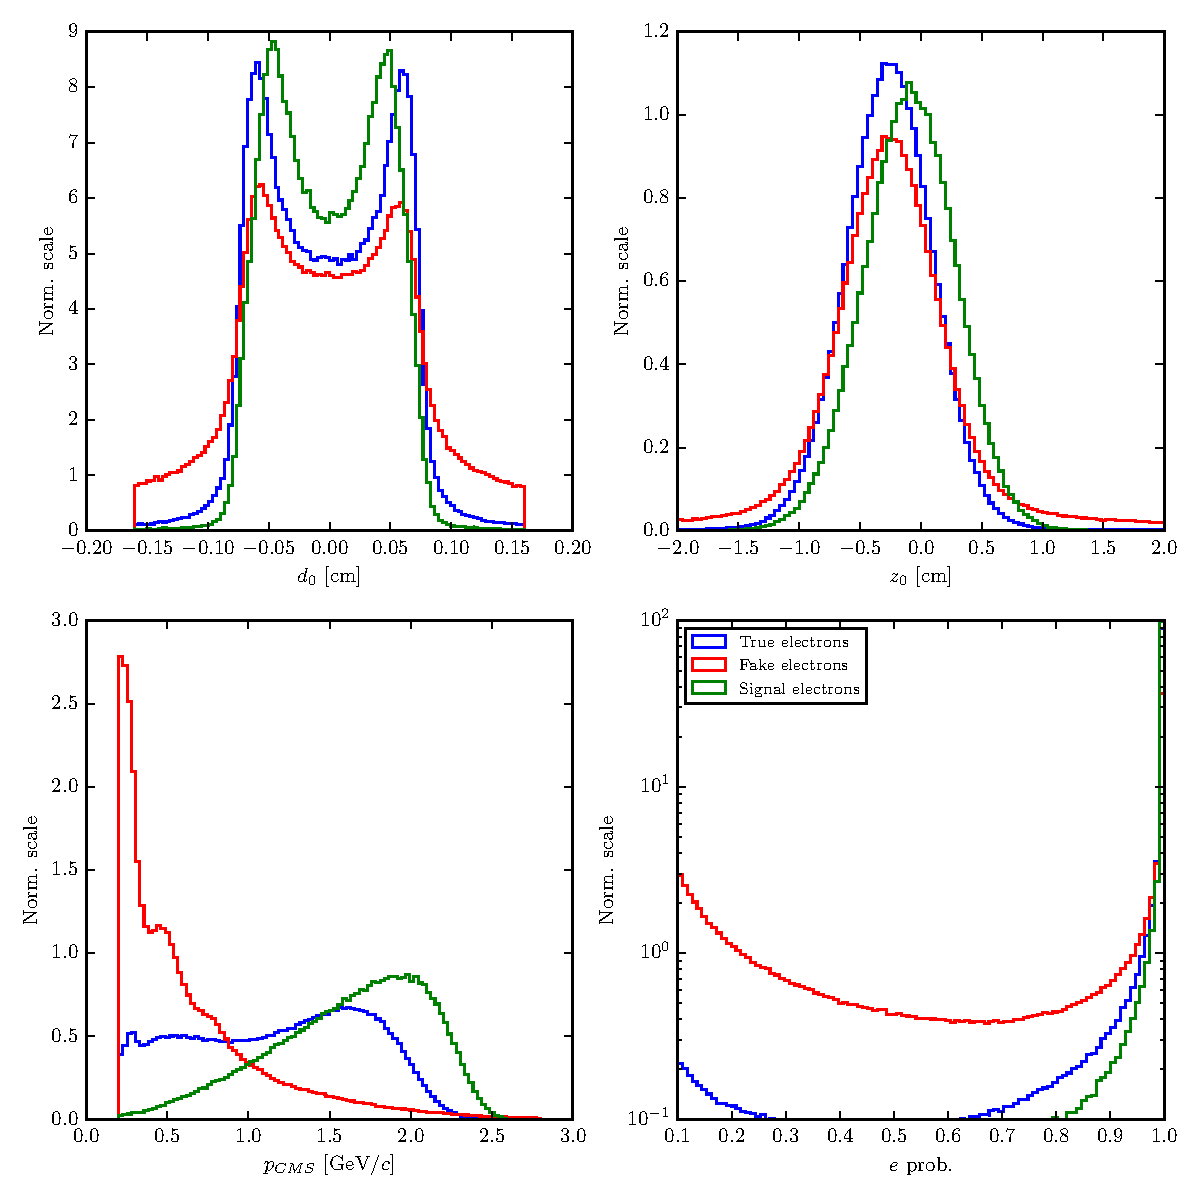
\includegraphics[width=\linewidth]{fig/FSP_e_vars}
\captionsetup{width=.8\linewidth}
\caption{Normalized properties of true (blue), fake (red) and true electrons (green) from signal decay}.
\label{fig:evars}
\end{figure}

\begin{figure}[H]
\centering
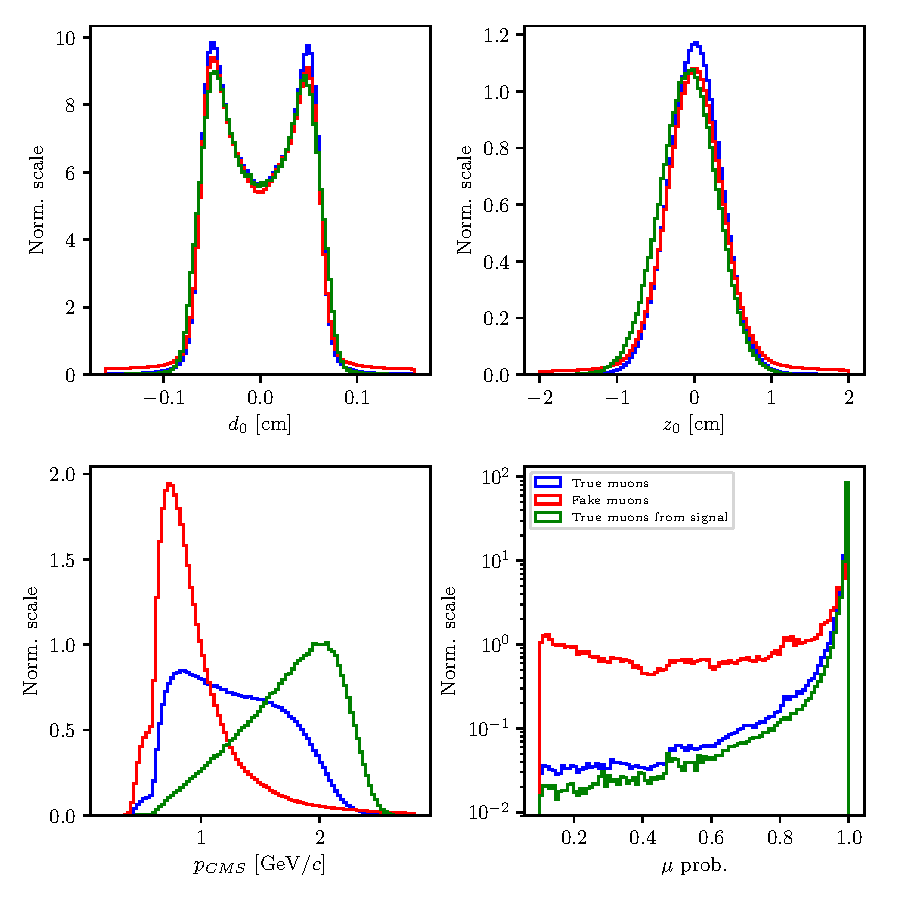
\includegraphics[width=\linewidth]{fig/FSP_mu_vars}
\captionsetup{width=.8\linewidth}
\caption{Normalized properties of true (blue), fake (red) and true muons (green) from signal decay}.
\label{fig:muvars}
\end{figure}

Based on the first plots, we can define a set of cuts:
\begin{itemize}
\item $\vert d_0 \vert < 0.1\e{cm}$,
\item $\vert z_0 \vert < 1.5\e{cm}$,
\item $p_{LAB} > 0.6\e{GeV}/c$ and $p_{CMS} \in [0.4,\,2.6]~\e{GeV}/c$ for electrons,
\item $p_{CMS} \in [0.6,\,2.6]~\e{GeV}/c$ for muons,
\end{itemize}

where the $p_{LAB}$ momentum cut for the electron case is chosen to discard a region with a sharp jump, which is assumed to come from sources like hard coded values in Belle software.

With this selection we can now determine the optimal PID cuts for electrons and muons, where we optimize with the standard definition of \textit{figure of merit} (FOM), shown in Figures \ref{fig:efom} and \ref{fig:mufom}. The cuts are optimized in steps of $0.1$, since we will later need to apply the PID correction factors, which are only available for cuts of these values.

\begin{equation}
\label{eq:fom}
FOM = \frac{S}{\sqrt{S+B}},
\end{equation} 
where $S$ represents number of signal and $B$ the number of background candidates.

\begin{figure}[H]
\centering
\captionsetup{width=.8\linewidth}
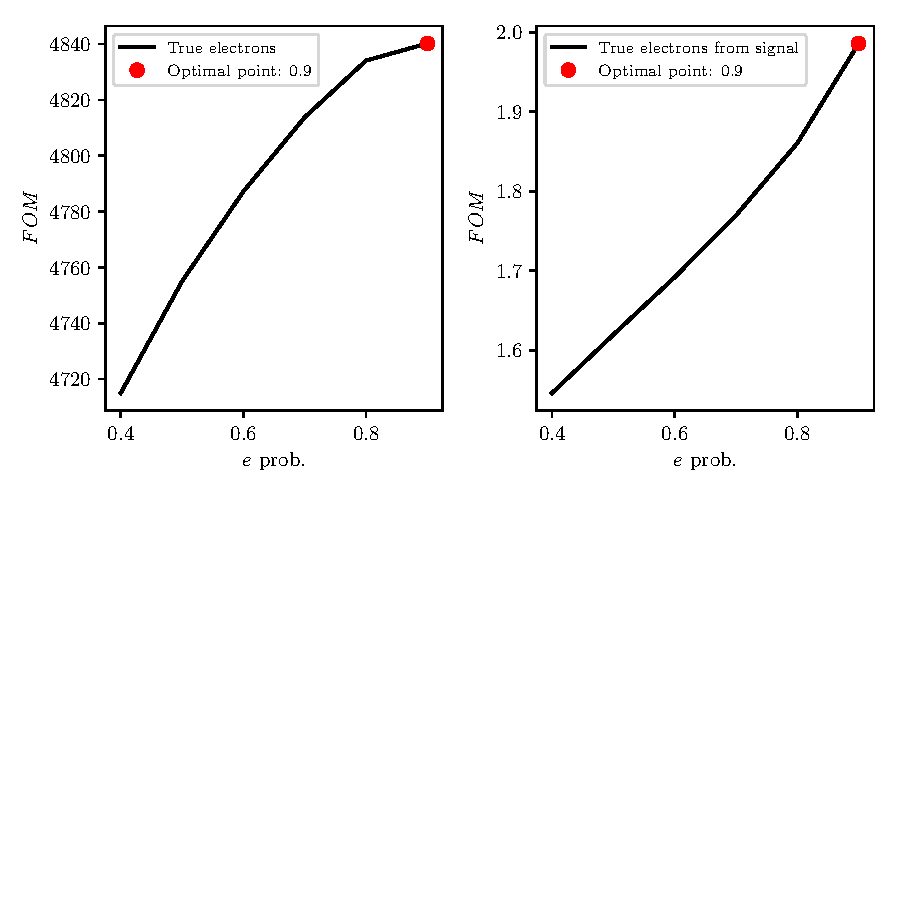
\includegraphics[width=\linewidth]{fig/FSP_e_fom}
\caption{$FOM$ optimizations of the PID probability cuts for true electrons (left) and true electrons from signal decays (right).}
\label{fig:efom}
\end{figure}

\begin{figure}[H]
\centering
\captionsetup{width=.8\linewidth}
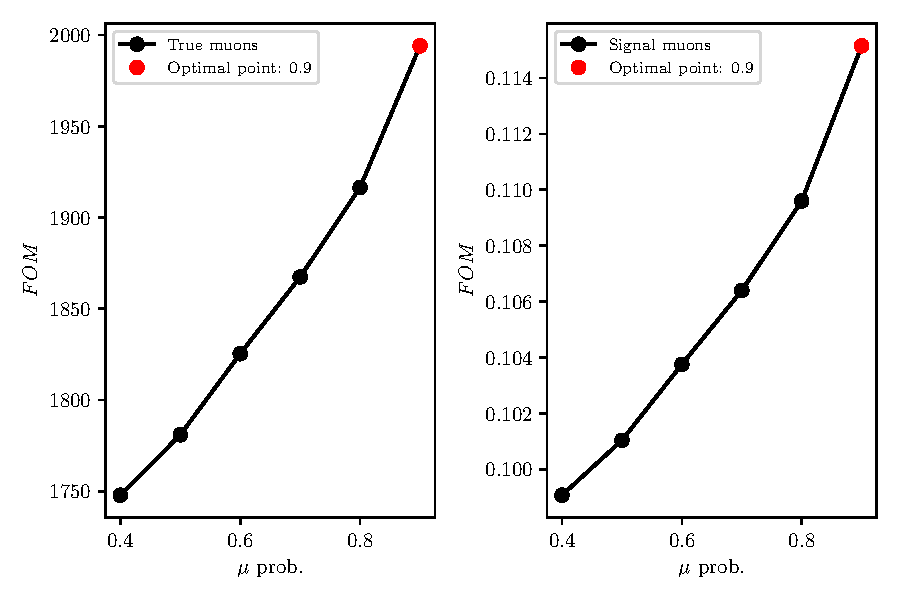
\includegraphics[width=\linewidth]{fig/FSP_mu_fom}
\caption{$FOM$ optimizations of the PID probability cuts for true muons (left) and true muons from signal decays (right).}
\label{fig:mufom}
\end{figure}

The optimized PID cuts for leptons are
\begin{itemize}
\item $e$ prob. $ > 0.9$ for electrons,
\item $\mu$ prob. $ > 0.9$ for muons.
\end{itemize}

The optimal value for the PID cuts is the same for all true leptons, if they are coming from signal decays or not, so this cut can be widely used on leptons coming from either $B$ meson in our analysis.

\subsubsection{Kaons}

For the case of kaons, the procedure is the same and the cuts are very similar. Figure \ref{fig:Kvars} shows the impact parameters $d_0$ and $z_0$, the momentum in  $\Upsilon(4S)$ center-of-mass system (CMS), and the PID information for true and fake kaons, where an extra category for true kaons from the signal decay is shown.

\begin{figure}[H]
\centering
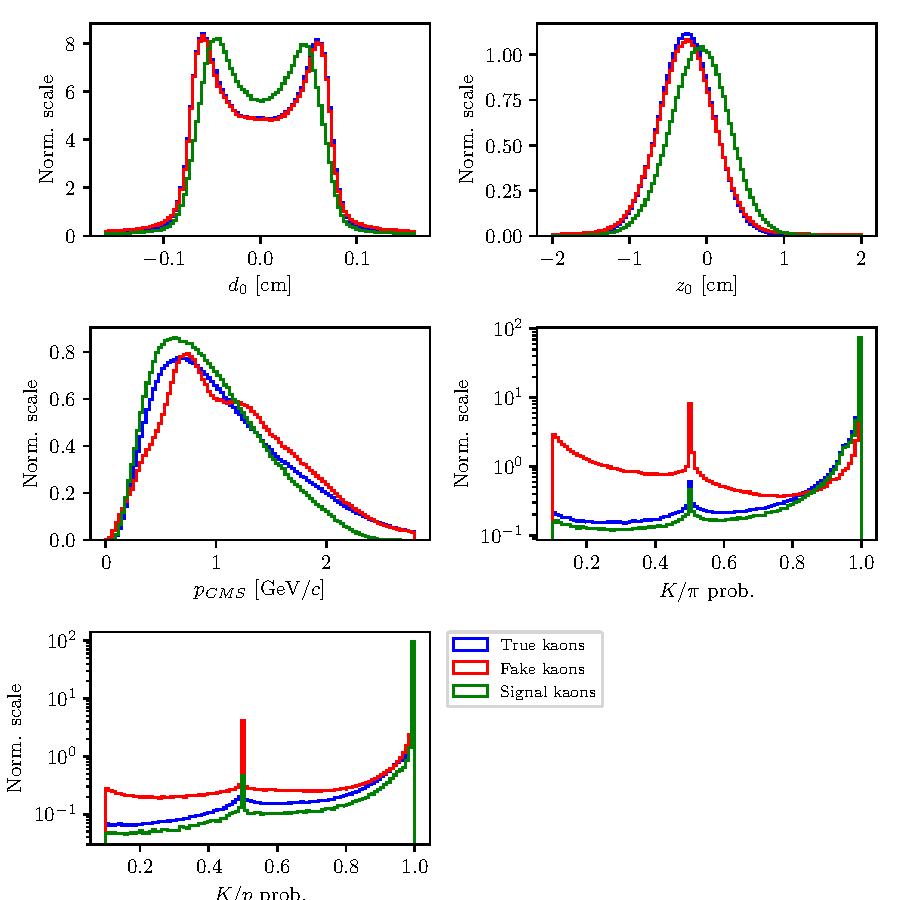
\includegraphics[width=\linewidth]{fig/FSP_kaon_vars}
\captionsetup{width=.8\linewidth}
\caption{Normalized properties of true (blue), fake (red) and true kaons (green) from signal decay}.
\label{fig:Kvars}
\end{figure}

We define the kaon cuts in the same manner as in the case for leptons
\begin{itemize}
\item $\vert d_0 \vert < 0.15\e{cm}$,
\item $\vert z_0 \vert < 1.5\e{cm}$,
\item $p_{CMS} \in [0,\,2.5]~\e{GeV}/c$.
\end{itemize}

The PID optimization in this case is taken in two steps. First we optimize the cut on $K / \pi$, and after that the $K/p$ separation probability. Figure \ref{fig:Kfom} shows the optimization procedure for PID cuts on kaon candidates.

\begin{figure}[H]
\centering
\captionsetup{width=.8\linewidth}
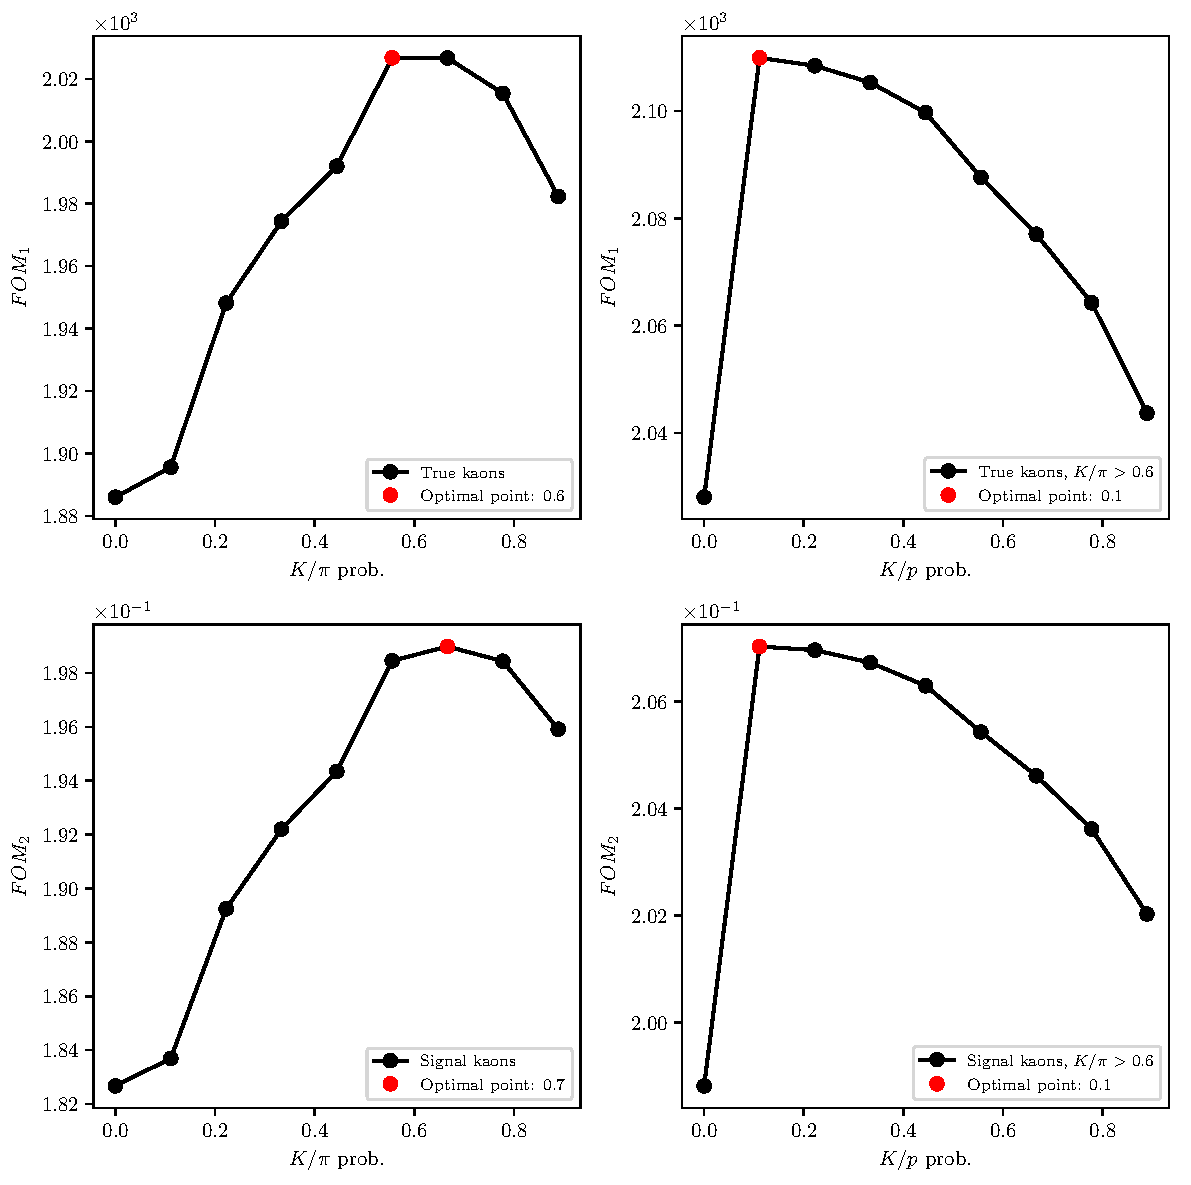
\includegraphics[width=\linewidth]{fig/FSP_kaon_fom}
\caption{$FOM$ optimizations of the PID probability cuts for true kaons (top) and true kaons from signal decays (bottom). The plots on the left show the optimization of the first step for the $K / \pi$ probability cut, and the plot on the right the $K/p$ probability cut.}
\label{fig:Kfom}
\end{figure}

The optimized PID cuts for kaons are
\begin{itemize}
\item $K/\pi > 0.7$,
\item $K/p > 0.3$.
\end{itemize}

\section{Combination of FSP particles}

With the pre-selected kaon and lepton candidates we make appropriate combinations for potential $B^+$ meson candidates. Due to our inability to reconstruct the neutrino, we are only able, at this point, to reconstruct the $B$ mesons in the following two channels
\begin{align*}
B^+ &\to K^+ K^- e^+, \\
B^+ &\to K^+ K^- \mu^+,
\end{align*}

and similarly for $B^-$. In order to further guarantee the proper combination of FSP particles, we perform a vertex fit of the three tracks. $B$ mesons have a relatively long lifetime, so they travel and decay along the z-axis of the detector in the direction of the boost, so we perform the vertex fit with an \textit{iptube} constraint, which constrains the vertex to an elongated ellipsoid along beam direction. We demand that the fit converged and apply a cut on the fit probability. The fit probability for signal and background $B$ meson candidates is shown in Figure \ref{fig:vtx} (left). We perform a $FOM$ cut optimization of this variable, which is shown in Figure \ref{fig:vtx} (right).

\begin{figure}[H]
\centering
\captionsetup{width=0.8\linewidth}
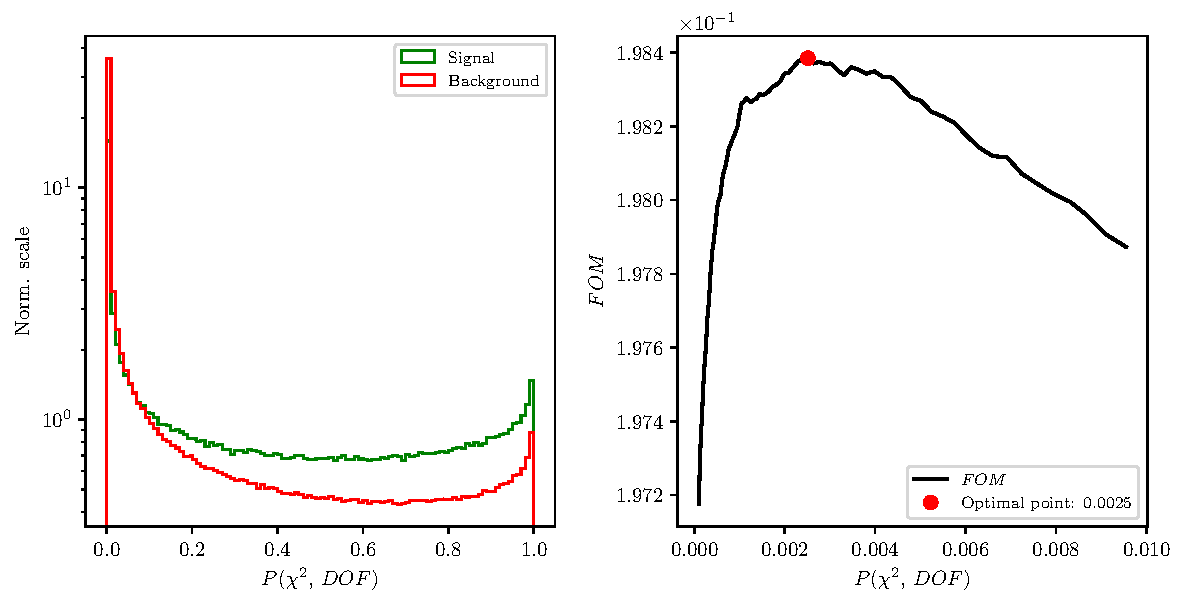
\includegraphics[width=\linewidth]{fig/VTX}
\caption{Normalized vertex fit probability distribution for signal and background $B$ meson candidates in logarithmic scale (left) and $FOM$ optimization of the vertex fit probability (right).}
\label{fig:vtx}
\end{figure}

The resulting vertex fit probability cut is then
\begin{itemize}
\item $P(\chi^2,NDF) > 4\times 10^{-3}$.
\end{itemize}

With the neutrino being the only missing particle on the reconstructed side, it is possible to determine the angle between the direction of the reconstructed $B$ (denoted as $Y \to K K \ell$) and the true $B$, as
\begin{align}
\mathrm{p}_\nu &= \mathrm{p}_B - \mathrm{p}_{Y}, \\
\label{eq:massnu}
\mathrm{p}_\nu^2 = m_\nu^2 &= m_B^2 + m_Y^2 - 2E_BE_Y + 2\vec{p}_B \cdot \vec{p}_Y \approx 0, \\ 
\label{eq:cosby}
\cos \left(\theta_{BY}\right) &= \frac{2E_BE_Y - m_B^2 - m_Y^2}{2\vert \vec{p}_B \vert \vert \vec{p}_Y\vert},
\end{align} 

where all the energy and momenta above are calculated in the CMS frame. The mass of the neutrino equals to 0 to a very good precision, so we used it in Eq. (\ref{eq:massnu}). In addition, we can substitute the unknown energy and momentum magnitude, $E_B$ and $\vert \vec{p}_B \vert$, of the $B$ meson in Eq. (\ref{eq:cosby}), with quantities from the well known initial conditions
\begin{align}
E_B &= E_{CMS} / 2,\\
\vert \vec{p}_B \vert = p_B &= \sqrt{E_B^2 - m_B^2},
\end{align} 

where $E_{CMS}$ is the total energy of the $e^+e^-$ collision in the CMS frame and $m_B$ is the nominal mass of the $B$ meson. 

For the correctly reconstructed candidates, this variable lies in the $[-1,1]$ region, though only to a certain precision, due to the finite detector resolution. For background candidates, however, the values populate also the non-physical regions, as is shown in Figure \ref{fig:cosby} (left). We impose an optimized cut on this variable from Figure \ref{fig:cosby} (right) to discard a large amount of background.
\begin{itemize}
\item $\vert \cos \left(\theta_{BY}\right) \vert < 1.0$.
\end{itemize}

\begin{figure}[H]
\centering
\captionsetup{width=.8\linewidth}
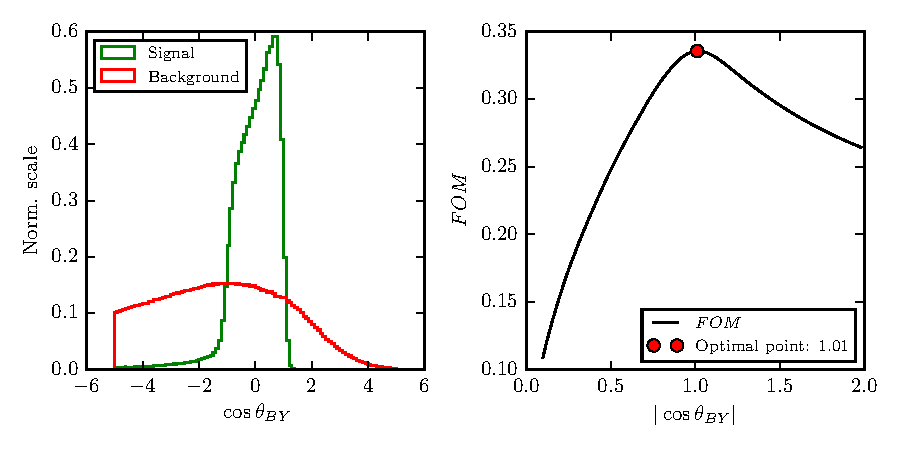
\includegraphics[width=\linewidth]{fig/cosBY}
\caption{Normalized $\cos \theta_{BY}$ distribution for signal and background $B$ meson candidates (left) and $FOM$ optimization of the $\cos \theta_{BY}$ variable (right).}
\label{fig:cosby}
\end{figure}

\section{Rest of event clean-up}
\label{sc:shortroe}

Due to the beam background in the detector, material interactions, or other processes, random tracks and clusters enter our event and get reconstructed as part of the physics process we want to study. These tracks and clusters are not interesting and further spoil the data we measure. In order to remedy this, we perform an extensive clean-up of the tracks and clusters in the ROE side, before calculating the four-momentum of the missing neutrino. The clean-up procedure is performed separately on tracks and clusters and uses multiple steps with multivariate analysis (MVA) algorithms in order to separate good tracks and clusters from the bad ones, which populate the ROE. Then, for each ROE object, a ROE mask is created for tracks and clusters, which is used to narrate the use of this track or cluster in the final calculations of the ROE four-momentum.

In order to preserve the continuity of this chapter, a more detailed description of the ROE clean-up can be found in Chapter \ref{ch:roe}. From this point on in this chapter the reader can assume the ROE to be clean.

\section{Loose neutrino reconstruction}

The signal-side neutrino escapes detection, so we cannot directly determine it's four-momentum. However, due to the detectors geometry, which almost completely covers the full solid angle, and due to well known initial conditions of the $\Upsilon(4S)$ meson, it is possible to determine the kinematics of the missing neutrino via indirectly reconstructing the other $B$ meson by summing up all the FSP particles four-momenta in the ROE. This is known as the \textit{untagged} method. Here we see the motivation for the ROE clean-up. If we did not depend on the other $B$ meson for our signal candidate reconstruction, this would not have been an issue.

The total missing four-momentum in the event can be determined as
\begin{align}
\mathrm{p}_{miss} &= \mathrm{p}_{\Upsilon(4S)} - \sum_i^{\mathrm{Event}}\left(E_i,\,\vec{p}_i \right),\\
\mathrm{p}_{miss} &= \mathrm{p}_{\Upsilon(4S)} - \left(\mathrm{p}_{Y} -\sum_i^{\mathrm{Rest~of~event}}\left(E_i,\,\vec{p}_i \right)\right).
\end{align}

where the summation runs over all charged and neutral particles in the defined set. We define the square of the missing mass, $m_{miss}^2$, which is zero, if signal side neutrino is the only missing particle in the event, as shown in Equation (\ref{eq:m2def}).
\begin{align}
\label{eq:nuold}
\mathrm{p}_\nu &= \mathrm{p}_{miss} = \left(E_{miss},\,\vec{p}_{miss} \right),\\
\label{eq:m2def}
m_{miss}^2 &= \mathrm{p}_{miss}^2 = \mathrm{p}_{\nu}^2 = m_\nu^2 \approx 0.
\end{align}

Since the detector is not perfect, the distribution of the $m_{miss}^2$ variable has a non-zero width. Additionally, tails are introduced as soon as we have additional missing particles such as extra missing neutrinos or other neutral undetected particles such as $K_L^0$, or simply missing tracks due to detection failure. Figure X shows the distribution of $m_{miss}^2$ as defined with the missing four-momentum in Eq. (\ref{eq:nuold}). Correctly reconstructed candidates, which come from events where the other $B$ meson decayed via a hadronic decay mode, should peak at zero. If this is not the case, candidates are shifted to larger values of this variable, as shown in Figure \ref{fig:missm2}. Due to this fact, we impose a cut on the $m_{miss}^2$ variable in order to discard all candidates with spoiled properties, even if it was in principle a correct combination of FSP particles on the signal side, in order to cut away events with a higher probability of a semi-leptonic decay of the other $B$ meson
\begin{itemize}
\item $\vert m_{miss}^2 \vert < 7\e{GeV}/c^2$.
\end{itemize}
This cut was not optimized, since the optimal case is considered to be too strong at this point in the analysis, since we still may want to attain as much signal candidates as possible, even if they are coming from events with semi-leptonic decays of the other $B$ meson.

For further purposes in this analysis we also define a subset of all signal candidates, which come from events where the other $B$ meson decayed hadronically and all of it's particles were taken into account correctly\footnote{We only allow for missing photons, since all photons are much harder to correctly take into account.}. We denote this subset as \textit{perfect} signal and the rest as \textit{non-perfect} signal.

\begin{figure}[H]
\centering
\captionsetup{width=.8\linewidth}
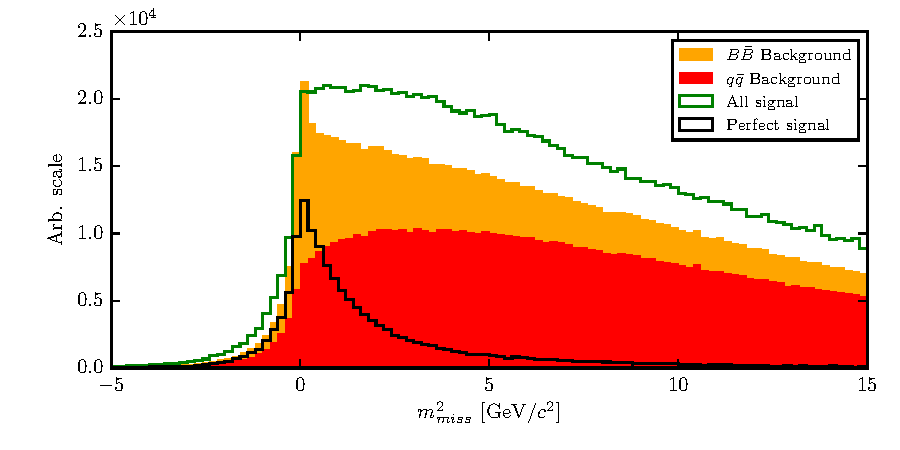
\includegraphics[width=\linewidth]{fig/missM2}
\caption{Normalized $\cos \theta_{BY}$ distribution for signal and background $B$ meson candidates (left) and $FOM$ optimization of the $\cos \theta_{BY}$ variable (right).}
\label{fig:missm2}
\end{figure}

The main uncertainty in neutrino four-momentum, defined as in Eq. (\ref{eq:nuold}) comes from energy uncertainty. It is a common practice to substitute the missing energy with the magnitude of the missing momentum, since the momentum resolution from the measurement is much better, thus redefining the neutrino four-momentum to
\begin{equation}
\label{eq:nunew}
\mathrm{p}_\nu = \left(\vert \vec{p}_{miss} \vert,\,\vec{p}_{miss} \right).
\end{equation}

The newly defined neutrino four-momentum can be added to the four-momentum of the $Y(KK\ell)$ candidate to obtain the full $B$ meson four-momentum and calculate the traditional $M_{BC}$ and $\Delta E$ variables
\begin{align}
\label{eq:de}
\Delta E &= E_B - E_{CMS}/2,\\
M_{BC} &= \sqrt{\left(E_{CMS}/2\right)^2 - \vert \vec{p} \vert^2}.
\end{align}

Since the final fit will be performed on these two variables, we define two regions
\begin{itemize}
\item Fit region: $M_{BC} \in [5.1,\,5.3]\e{GeV}/c^2$ and $\Delta E \in [-1.3,\,1,5]\e{GeV}$,
\item Signal enhanced region: $M_{BC} \in [5.27,\,5.3]\e{GeV}/c^2$ and $\vert \Delta E \vert < 0.166 \e{GeV}$,
\end{itemize}

where the signal enhanced region was defined via a 2D $FOM$ optimization on the perfectly reconstructed signal candidates, shown on Figure X. Figure \ref{fig:mbc_de_pre} shows the distributions of $\Delta E$ (left) and $M_{BC}$ (right) for signal and major types of background after the precuts. Both signal components are scaled up with respect to the background components, but are in proper scale one to another. The effects of missing particles are clearly seen on both distributions even for signal candidates.

\begin{figure}[H]
\captionsetup{width=0.8\linewidth}
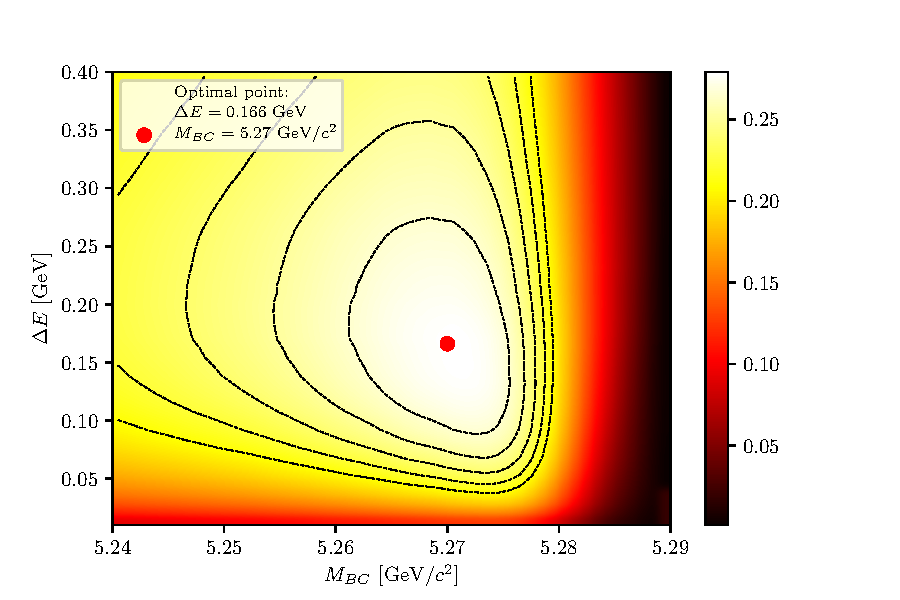
\includegraphics[width=\linewidth]{fig/sigWin}
\caption{2D $FOM$ optimization of the signal window definition, where the signal in the optimization was represented by perfectly reconstructed candidates.}
\label{fig:sigwin}
\end{figure}

\begin{figure}[H]
\captionsetup{width=0.8\linewidth}
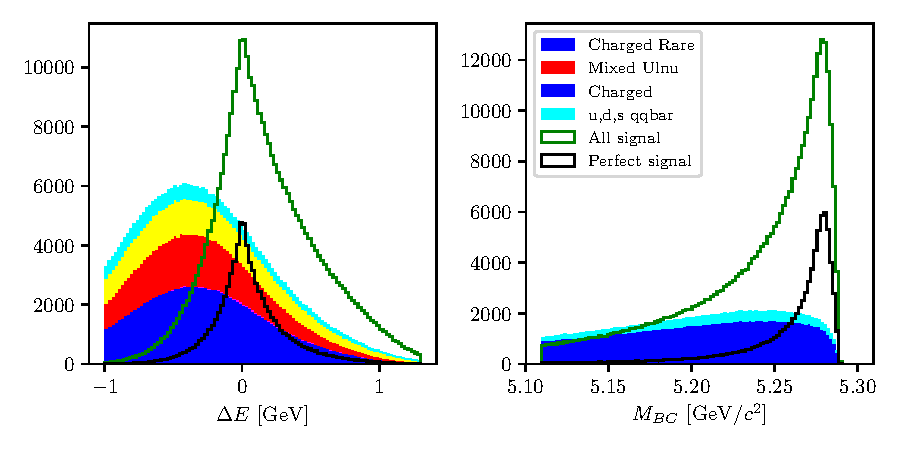
\includegraphics[width=\linewidth]{fig/mbc_de_pre}
\caption{Distributions of $\Delta E$ (left) and $M_{BC}$ (right) for signal and major types of background after the precuts. Both signal components are scaled up with respect to the background components, but are in proper scale one to another. The perfect signal has a much better resolution in both distributions, since the event is perfectly reconstructed.}
\label{fig:mbc_de_pre}
\end{figure}


\section{$q^2$ calculation}

Momentum transfer squared, $q^2$, is the squared Lorentz invariant of the four-momentum which is transferred from the $B$ meson to the $W$ boson. There are several possible calculations of this variable which offer different resolution. The following describes the calculation of $q^2$ which follows the calculation from [] and yields the best resolution.

For correctly reconstructed events, Eq. (\ref{eq:de}) should satisfy the condition $\Delta E \approx 0$ within precision. It is possible to rescale the neutrino energy in such way that we fix $\Delta E$ to zero, meaning 
\begin{equation}
\Delta E' = (E_Y + \alpha E_\nu) - E_{CMS}/2 = 0.
\end{equation}
and calculate and adapted version of $M_{BC}$
\begin{equation}
M_{BC}' = \sqrt{\left(E_{CMS}/2\right)^2 - \vert \vec{p}_Y + \alpha \vec{p}_\nu \vert^2}.
\end{equation}

The neutrino momentum resolution dominates the $\Delta E$ uncertainty [], so the correction factor $\alpha$ reduces this source of uncertainty. Additionally, it reduces the correlations between $\Delta E$ and $M_{BC}'$, so the latter variable might be the better choice thank $M_{BC}$ in the final extraction fit. 

A second correction can be applied by rotating the direction of the neutrino momentum by a small angle with respect to the reconstructed one. Such an angle is chosen in order fix the value of $M_{BC}'$ to the nominal mass of the $B$ meson, $m_B$.

The corrected neutrino momentum is then solely used for the $q^2$ calculation, alongside the reconstructed lepton four-momentum, as
\begin{equation}
\label{eq:q2}
q^2 = \mathrm{q}^2 = \left(\mathrm{p}_\ell + \mathrm{p}_\nu \right)^2.
\end{equation}

The $q^2$ distribution and its resolution are shown in Figure \ref{fig:q2}, along with additional versions of $q^2$, with details of the calculation method in the caption.

\begin{figure}[H]
\captionsetup{width=0.8\linewidth}
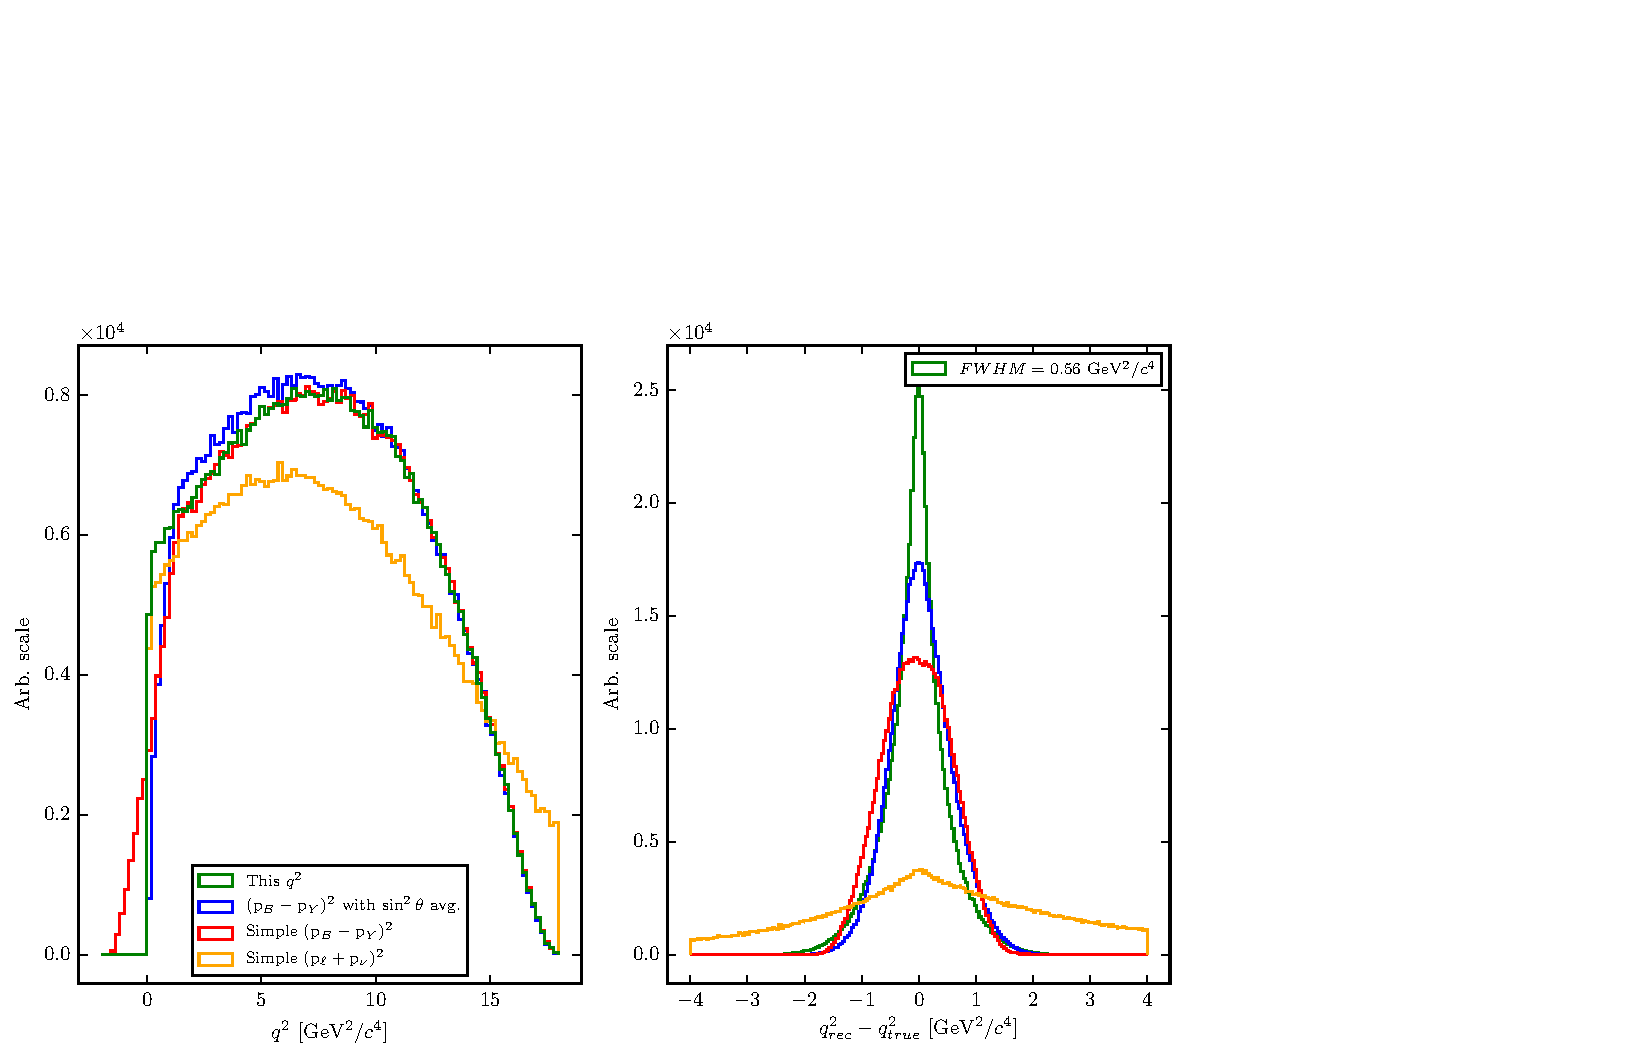
\includegraphics[width=\linewidth]{fig/q2}
\caption{Distributions of $q^2$ (left) and $q^2$ resolution (right) for various methods of $q^2$ calculation. The blue distribution follows the procedure in [], whereas the red and the orange ones are straight-forward calculations with available information in the reconstruction. The $q^2$ calculation in red assumes a resting $B$ meson in the CMS frame, and the calculation in orange uses the neutrino four-momentum from Eq. (\ref{eq:nuold}).}
\label{fig:q2}
\end{figure}

However, this says nothing about the correctness of the $q^2$ model which was used (ISGW2). Since this decay has not been observed yet, we do not have a good description of the decay model, which is also a source of systematics in this analysis.

\section{Selection summary}

In this section one can find the summary of all selection cuts in the event reconstruction, from FSP particles up to the $B$ meson.

\begin{itemize}
\item FSP particles
	\begin{itemize}
	\item Electrons: $\vert d_0 \vert < 0.1\e{cm},\,\vert z_0 \vert < 1,5\e{cm},\,p>0.6\e{GeV}/c,\\p_{CMS}\in[0.4,\,2.6]\e{GeV}/c,\,eID>0.9$
    \item Muons: $\vert d_0 \vert < 0.1\e{cm},\,\vert z_0 \vert < 1,5\e{cm},\,p_{CMS}\in[0.6,\,2.6]\e{GeV}/c,\\\mu ID>0.9$
    \item Kaons: $\vert d_0 \vert < 0.15\e{cm},\,\vert z_0 \vert < 1,5\e{cm},\,p_{CMS} < 2.5\e{GeV}/c,\\K/\pi~ID>0.6$
	\end{itemize}
\item $B$ mesons:
	\begin{itemize}
	\item $P(\chi^2,\,DOF) > 4\times10^{-3},\,\vert \cos \theta_{BY} \vert < 1,\,\vert m_{miss}^2 \vert < 7\e{GeV}/c^2,\\\Delta E \in [-1.3,1.5]\e{GeV},\,M_{BC} > 5.1\e{GeV}/c^2.$
	\end{itemize}
\end{itemize}

\chapter{Rest of event clean-up}
\label{ch:roe}

Continuing from Section \ref{sc:shortroe}, the description of the ROE clean-up process is described here. 

\section{Setting up the MVA}

Training the MVA classifiers follows the same recipe for all the steps. For each step we run our $B$ meson reconstruction on Signal MC with a generic companion $B$ meson. This way the produced weight files are less likely to be dependent on the signal side and can be used also for untagged analyses of other decays. For every correctly reconstructed signal $B$ meson we save the necessary information for each MVA step (i.e. properties of ROE clusters). Only correctly reconstructed candidates are chosen here, to prevent leakage of information from the signal side to the ROE side.

For each cleanup-step a dataset of $2\times N$ was prepared for the training of "signal" against "background". The dataset for each case was split into 5 parts for reasons which are explained later on in the note. The Fast-BDT (FBDT) [] algorithm was used as the MVA method, where the following hyper-parameters were optimized with a grid search
\begin{itemize}
\item \texttt{nTrees}: the number of trees in the FBDT forest,
\item \texttt{nLevels}: the number of levels in each FBDT tree.
\end{itemize}

Figure X shows a graphical interpretation of the FBDT forest with \texttt{nTrees} and \texttt{nLevels}. In all cases the hyper-parameters were optimized with a grid search in the hyper-parameter space. Additionally, we perform a $k$-fold cross-validation ($k=5$) for each hyper-parameter set, where we cycle through the $5$ parts of the dataset and $4$ parts of the dataset are used for training, whereas the remaining part is used for validation. This minimizes the bias towards the validation sample when optimizing the hyper-parameters. Figure X shows a schematic procedure of a $k$-fold cross-validation.

\section{Clusters clean-up}

Generally speaking, most of the photons in $B$-physics should come from $\pi^0 \to \gamma \gamma$ decays. However, a lot of clusters are also created by photons coming from the beam background or interactions with the detector material. These photons add extra energy and momentum which we then measure.

In the first step of the clusters clean-up we train an MVA which recognizes good $\pi^0$ candidates. The output of this classifier is then applied to photons and represents a sort of a $\pi^0$ probability, which is used as an additional classifier variable in the next step of the clean-up, where we train an MVA to separate good photon clusters from bad ones.

\subsection{$\pi^0$ MVA training}

The dataset of $\pi^0$ candidates contains
\begin{itemize}
\item 387125 signal candidates,
\item 416019 background candidates,
\end{itemize}
where the definition of signal is that both photon daughters that were used in the reconstruction of the $\pi^0$ are actual photons and actual daughters of the particle, based on the MC truth. We use $\pi^0$ candidates from the converted $\pi^0$ particle list from Belle MC with the invariant mass in the range of $M \in [0.10,~0.16]\e{GeV}$ and perform a mass-constrained fit on all candidates, keeping only the cases where the fit converged. 

The input variables used in this MVA are
\begin{itemize}
\item $p$ and $p_{CMS}$ of $\pi^0$ and $\gamma$ daughters,
\item $P(\chi^2,NDF)$ of the mass-constrained fit, invariant mass and significance of mass before and after the fit,
\item angle between the daughter photons in CMS frame,
\item cluster quantities for each daughter photon
	\begin{itemize}
	\item $E_9/E{25}$,
	\item theta angle,
	\item number of hit cells in the ECL,
	\item highest energy in cell,
	\item energy error,
	\item distance to closest track at ECL radius.
	\end{itemize}
\end{itemize}

The classifier output variable is shown in Figure X.

\begin{center}
PLOT
\end{center}

The distributions for all input variables and their correlations for signal and background candidates can be found in Appendix X for all steps of the clean-up.


\subsection{$\gamma$ MVA training}

The dataset of $\gamma$ candidates contains
\begin{itemize}
\item 324781 signal candidates,
\item 333353 background candidates,
\end{itemize}
where the definition of signal is that the photon is an actual photon and that the related ECL cluster is related to a primary MC particle. This tags all photon particles from secondary interactions as background photons. We use $\gamma$ candidates from the converted $\gamma$ particle list from Belle MC. The $\pi^0$ probability information from the previous step is applied to all photon pairs which pass the same $\pi^0$ cuts as defined in the previous step. Since it's possible to have overlapping pairs, the $\pi^0$ probability is overwritten, if the new value is greater than the existing one, since this points to a greater probability of a correct $\pi^0$ combination.

The input variables used in this MVA are
\begin{itemize}
\item $p$ and $p_{CMS}$ of $\gamma$ candidates,
\item $\pi^0$ probability,
\item cluster quantities
	\begin{itemize}
	\item $E_9/E{25}$,
	\item theta angle,
	\item number of hit cells in the ECL,
	\item highest energy in cell,
	\item energy error,
	\item distance to closest track at ECL radius.
	\end{itemize}
\end{itemize}

The classifier output variable is shown in Figure X.

\begin{center}
PLOT
\end{center}

\subsection{Clusters clean-up optimization}

We now have the final weights for photon classification. We apply these weights to the photon particle list, coming from the generically decaying $B$ mesons with correctly reconstructed signal $B$ mesons on the other side. After applying the weights we optimize the cut based on the standard definition of the $FOM$. The cut optimization is shown in Figure X, with the optimal cut on the $\gamma$ classifier output at $X$.

\begin{center}
PLOT
\end{center}

Figure shows the LAB frame momentum of the photons before and after the cut in logarithmic scale. The signal efficiency and background rejection at this cut are
\begin{itemize}
\item Signal efficiency: $\epsilon_{SIG} = X$,
\item Background rejection: $1-\epsilon_{BKG} = X$.
\end{itemize}

\begin{center}
PLOT
\end{center}

\section{Tracks clean-up}

\chapter{Background suppression}




\end{document}


